
\chapter{Result Analysis}
\label{sec:result_analysis}

% \begin{figure}[htbp]
%     \centering
%     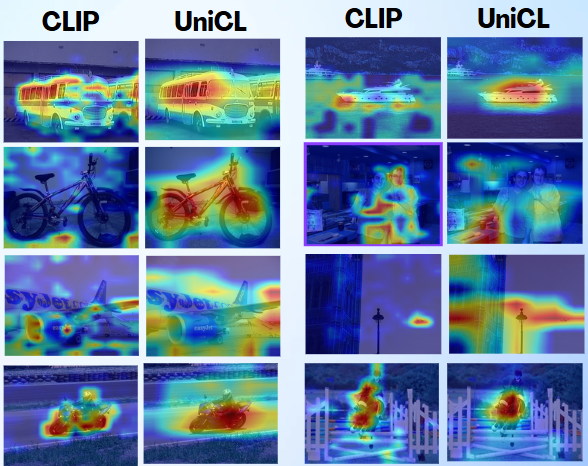
\includegraphics[width=0.8\textwidth]{clip_vs_unicl.png}
%     \caption{Quantitative analysis of CAMs produced by CLIP and Swin}
%     \label{fig:cam_results}
% \end{figure}

% \autoref{fig:cam_results} shows the comparison of the CAMs generated by CLIP \cite{vl_clip} and UniCL \cite{vl_unicl} on the Pascal VOC 2012 dataset. The results indicate that UniCL produces more accurate and detailed CAMs compared to CLIP. You can see the bicycle in second row, first two columns, CLIP even failed to detect it, while UniCL was localize it very well. The same is true for third and fourth columns of the same row, where CLIP failed to highlight the boat, but UniCL did.

% Additionally, we can see in all the images that, the CAMs produced by CLIP are discontinuous and sparse, while the CAMs produced by UniCL are more continuous and dense. This indicates that UniCL is better at capturing the global context of the image.

% However, we also observed that the CAMs produced by UniCL are still not perfect. It produces a lot of false positives, for example, look at the third row, last column, where it was supposed highlight an aeroplane, but it also highlighted the background. Also in some cases, like the last row, CLIP was able to trace the object boundary with better detail. This indicates that there is still room for improvement in the CAM generation process.

\section{Data and Experimental Setup}
\label{subsec:data_and_experimental_setup}

We conducted our experiments on the \textbf{Pascal VOC 2012} dataset \cite{dataset_pascal_voc}, 
which contains 20 object categories and one background class. 
The dataset is split into 1,464 training images, 1,449 validation images, 
and 1,456 test images. Since the test set does not provide ground truth 
annotations, we used the training set for model training and the validation 
set for performance evaluation.

All experiments were implemented in the \textbf{PyTorch} framework and executed 
on a single \textbf{NVIDIA Tesla T4 GPU} with \textbf{16 GB of memory}, 
provided by Google Colab (free tier). During training, images were randomly 
resized within the range of 512--2048 pixels, rescaled by factors between 
0.5 and 2.0, and cropped to a fixed size of 224.

Optimization was performed using the \textbf{AdamW} optimizer with a learning 
rate of $5 \times 10^{-5}$, $\beta_1 = 0.9$, $\beta_2 = 0.999$, and a weight 
decay of 0.01. We trained the models for \textbf{30,000 iterations} with an 
effective batch size of 8 (per-GPU batch size of 4 with gradient accumulation 
steps of 2). A linear warmup strategy was applied during the first 500 iterations 
with a warmup ratio of $10^{-3}$. The best-performing checkpoints were selected 
based on validation set performance.


\input{chapters/result_analysis/implementation_details.tex}

\section{Quantitative Results}
\label{subsec: Quantitative Results}
We compared the performance of our proposed method with the baseline method CLIP \cite{wsss_frozen_clip} on the Pascal VOC 2012 dataset. The results are shown in Table \ref{tab:quantitative_results}. Our proposed method outperforms the baseline method by a significant margin, achieving a mIoU of 55.4\% compared to 47.5\% for the baseline method. This demonstrates the effectiveness of our proposed method in generating accurate CAMs for weakly supervised semantic segmentation.

\begin{table}[ht]
    \centering
    \renewcommand{\arraystretch}{1.2}
    \setlength{\tabcolsep}{6pt}
    \begin{tabular}{l c c c c}
        \hline
        Method                                                               & Backbone   & Sup. & val           & test          \\
        \hline
        \multicolumn{5}{c}{\textit{multi-stage weakly supervised approaches}}                                                    \\
        RCA$_{\text{CVPR'22}}$~\cite{wsss_RCA}             & ResNet101  & I+S  & 72.2          & 72.8          \\
        L2G$_{\text{CVPR'22}}$~\cite{wsss_L2G}             & ResNet101  & I+S  & 72.1          & 71.7          \\
        Mat-label$_{\text{ICCV'23}}$~\cite{wsss_MatLabel}  & ResNet101  & I+S  & 73.3          & \textbf{74.0} \\
        S-BCE$_{\text{ECCV'22}}$~\cite{wsss_s_bce}         & ResNet38   & I+S  & 68.1          & 70.4          \\
        RIB$_{\text{NeurIPS'21}}$~\cite{wsss_rib}          & ResNet38   & I    & 68.3          & 68.6          \\
        W-OoD$_{\text{CVPR'22}}$~\cite{wsss_ood}      & ResNet101  & I    & 69.8          & 69.9          \\
        ESOL$_{\text{NeurIPS'22}}$~\cite{wsss_esol}   & ResNet101  & I    & 69.9          & 69.3          \\
        VML$_{\text{IJCV'22}}$~\cite{wsss_vml}        & ResNet101  & I    & 70.6          & 70.7          \\
        AETF$_{\text{ECCV'22}}$~\cite{wsss_aetf}      & ResNet38   & I    & 70.9          & 71.7          \\
        MCTformer$_{\text{CVPR'22}}$~\cite{wsss_MCTformer} & ViT+Res38  & I    & 70.4          & 70.0          \\
        CDL$_{\text{IJCV'23}}$~\cite{wsss_cdl}        & ResNet101  & I    & 72.4          & 72.2          \\
        ACR$_{\text{CVPR'23}}$~\cite{wsss_acr}        & ViT        & I    & 72.4          & 72.4          \\
        BECO$_{\text{CVPR'23}}$~\cite{wsss_beco}      & MIT-B2     & I    & 73.7          & 73.5          \\
        FPR$_{\text{ICCV'23}}$~\cite{wsss_fpr}        & ResNet101  & I    & 70.0          & 70.6          \\
        USAGE$_{\text{ICCV'23}}$~\cite{wsss_usage}    & ResNet38   & I    & 71.9          & 72.8          \\
        CLIMS$_{\text{CVPR'22}}$~\cite{wsss_clims}    & ViT+Res101 & I+L  & 70.4          & 70.0          \\
        CLIP-ES$_{\text{CVPR'23}}$~\cite{wsss_clip_es}                       & ViT+Res101 & I+L  & \textbf{73.8} & 73.9          \\
        \hline
        \multicolumn{5}{c}{\textit{single-stage weakly supervised approaches}}                                                   \\
        1Stage$_{\text{CVPR'20}}$~\cite{wsss_single_stage}                   & ResNet38   & I    & 62.7          & 64.3          \\
        RRM$_{\text{AAAI'20}}$~\cite{wsss_reliability_does_matter}           & ResNet38   & I    & 62.6          & 62.9          \\
        AA\&AR$_{\text{ACMMM'21}}$~\cite{wsss_aaar}                                 & ResNet38   & I    & 63.9          & 64.8          \\
        SLRNet$_{\text{IJCV'22}}$~\cite{34}                                  & ResNet38   & I    & 67.2          & 67.6          \\
        AFA$_{\text{CVPR'22}}$~\cite{39}                                     & MIT-B1     & I    & 66.0          & 66.3          \\
        TSCD$_{\text{AAAI'23}}$~\cite{53}                                    & MIT-B1     & I    & 67.0          & 67.5          \\
        ToCo$_{\text{CVPR'23}}$~\cite{40}                                    & ViT        & I    & 71.1          & 72.2          \\
        \hline
        ours-WeCLIP (w/o CRF)                                                & ViT        & I+L  & 74.9          & 75.2          \\
        ours-WeCLIP (w/ CRF)                                                 & ViT        & I+L  & \textbf{76.4} & \textbf{77.2} \\
        \hline
    \end{tabular}
    \caption{Comparison of multi-stage and single-stage weakly supervised approaches.}
    \label{tab:quantitative_results}
\end{table}

\section{Qualitative Analysis}
\label{sec:qualitative_analysis}

We present qualitative comparisons of our UniCL-AffSeg framework against the WeCLIP baseline and ground truth annotations on selected Pascal VOC 2012 images. Both class activation maps (CAMs) and pseudo-labels are visualized to highlight differences in object localization, boundary delineation, and overall mask quality.

% \subsection{Selection of Examples}
% The images were chosen to represent a variety of scenarios, including: 
% \begin{itemize}
%     \item \t	\textbf{Easy cases:} Large, isolated objects where CAMs are expected to cover most of the object region.
%     \item \t	\textbf{Challenging cases:} Small objects, occlusions, or cluttered backgrounds where weakly supervised CAMs often fail to capture complete object extents.
% \end{itemize}

% \subsection{Visualization Layout}
% Figure~\ref{fig:qualitative_comparison} shows the qualitative results in a structured grid. 
% The first row presents the input image, ground truth, WeCLIP CAM, and our CAM, while the second row shows the corresponding pseudo-labels generated by WeCLIP and our method. This layout allows a direct comparison of both intermediate activations and the resulting segmentation masks.


\begin{figure}[ht]
  \centering
  \setlength{\tabcolsep}{2pt} % adjust spacing
  \renewcommand{\arraystretch}{0.9}

  % Wrap the table in a colored box (requires \usepackage{tcolorbox})
  \begin{tcolorbox}[colframe=black!60, colback=white, boxrule=0.8pt, arc=2pt, left=2pt, right=2pt, top=2pt, bottom=2pt]
    \centering
    % CAMs with class labels on the left
    \begin{tabular}{m{3cm} c c c} % first column = label

      % Column headers
       & (a) Input                                                    & (b) WeCLIP & (c) Ours
      \\
      [1mm]

      {\textbf{Cat}}
       & 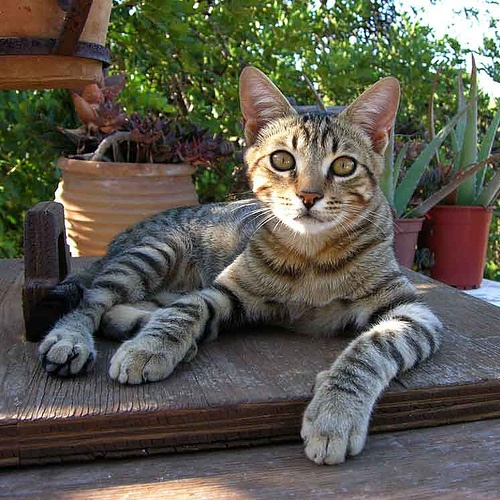
\includegraphics[width=0.20\textwidth,height=0.20\textwidth]
      {figures/originals/2007_003778}
       & 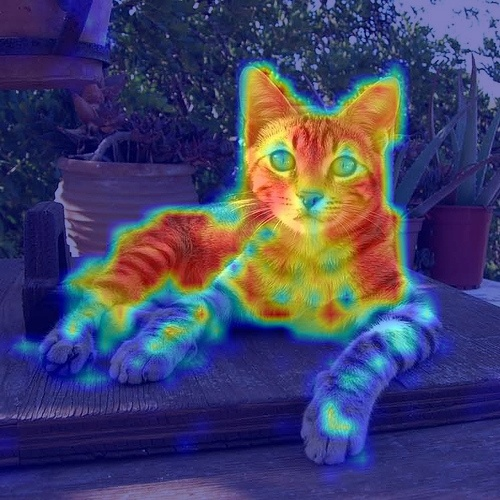
\includegraphics[width=0.20\textwidth,height=0.20\textwidth]
      {figures/val_cams/weclip/2007_003778_7}
       & 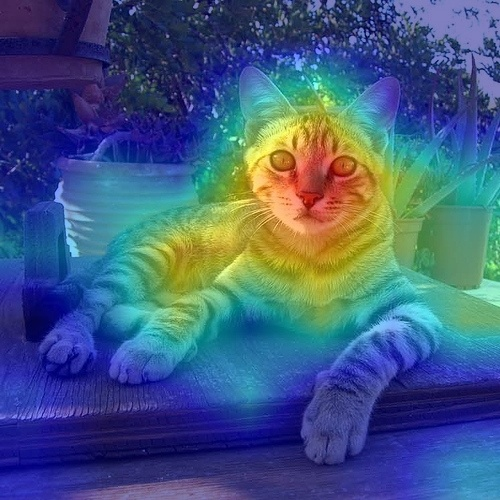
\includegraphics[width=0.20\textwidth,height=0.20\textwidth]
      {figures/val_cams/ours/2007_003778_7}
      \\
      \textbf{Bicycle}
       & 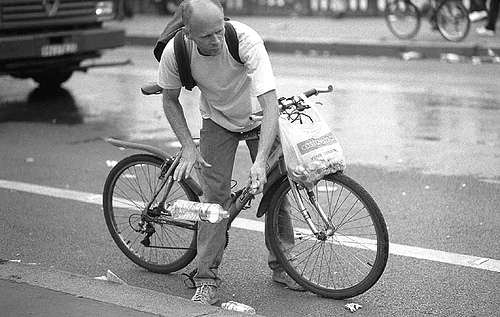
\includegraphics[width=0.20\textwidth,height=0.20\textwidth]
      {figures/originals/2011_000453}
       & 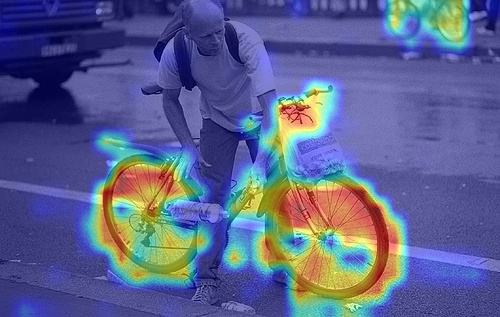
\includegraphics[width=0.20\textwidth,height=0.20\textwidth]
      {figures/val_cams/weclip/2011_000453_1}
       & 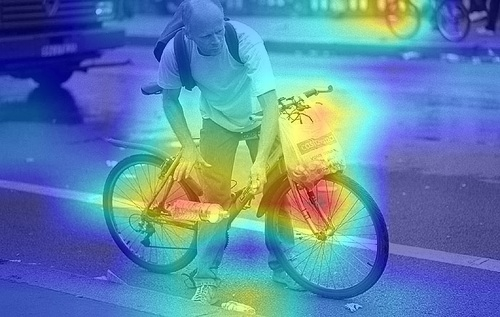
\includegraphics[width=0.20\textwidth,height=0.20\textwidth]
      {figures/val_cams/ours/2011_000453_1}
      \\
      \textbf{Bird}
       & 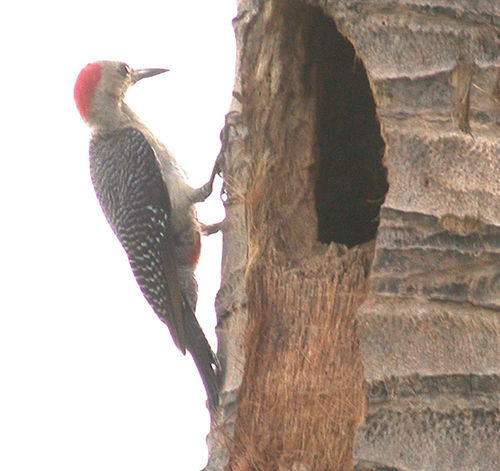
\includegraphics[width=0.20\textwidth,height=0.20\textwidth]
      {figures/originals/2011_001902}
       & 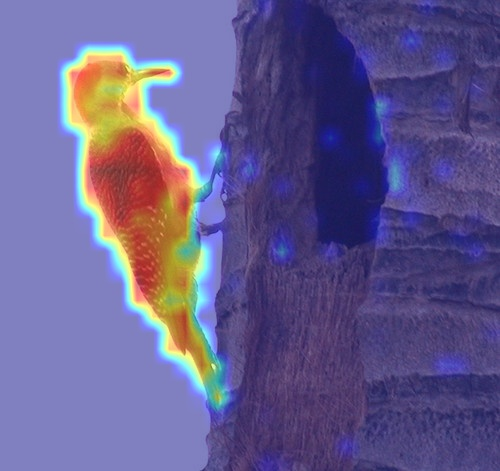
\includegraphics[width=0.20\textwidth,height=0.20\textwidth]
      {figures/val_cams/weclip/2011_001902_2}
       & 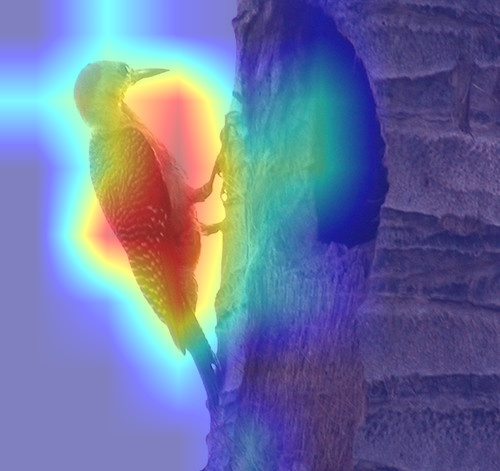
\includegraphics[width=0.20\textwidth,height=0.20\textwidth]
      {figures/val_cams/ours/2011_001902_2}
      \\
      \textbf{Boat}
       & 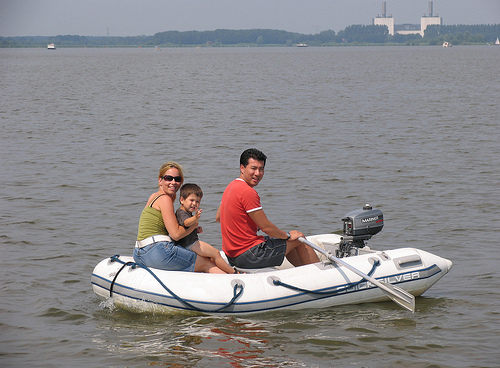
\includegraphics[width=0.20\textwidth,height=0.20\textwidth]
      {figures/originals/2010_003599}
       & 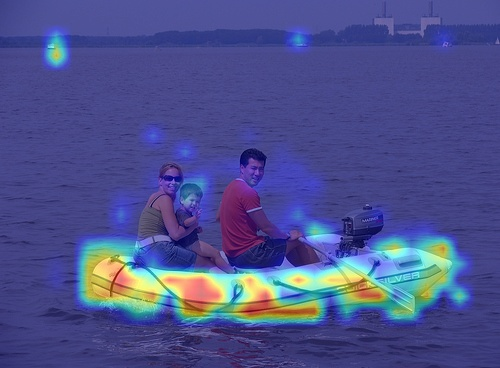
\includegraphics[width=0.20\textwidth,height=0.20\textwidth]
      {figures/val_cams/weclip/2010_003599_3}
       & 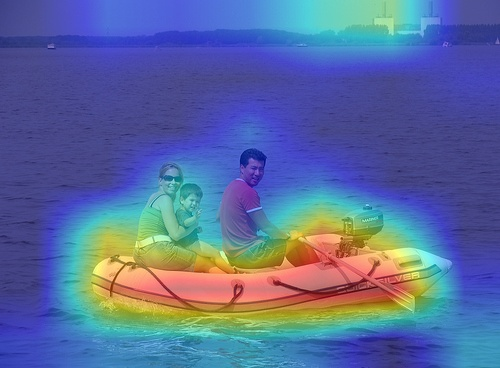
\includegraphics[width=0.20\textwidth,height=0.20\textwidth]
      {figures/val_cams/ours/2010_003599_3}
      \\
      \textbf{Pottedplant}
       & 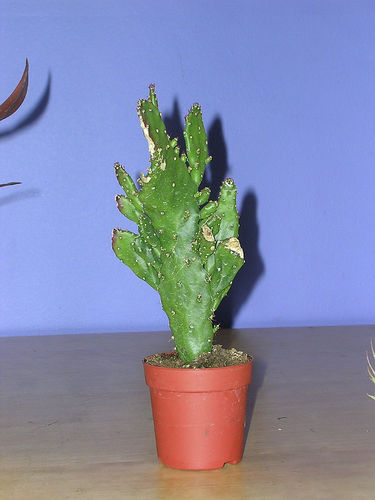
\includegraphics[width=0.20\textwidth,height=0.20\textwidth]
      {figures/originals/2011_000145}
       & 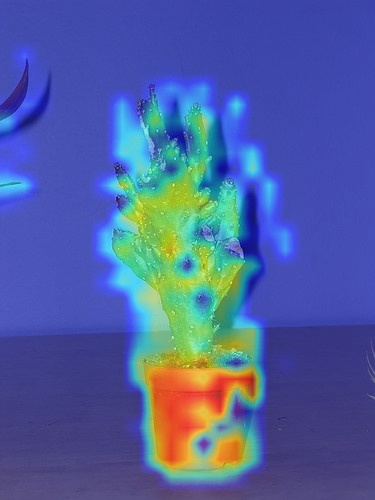
\includegraphics[width=0.20\textwidth,height=0.20\textwidth]
      {figures/val_cams/weclip/2011_000145_15}
       & 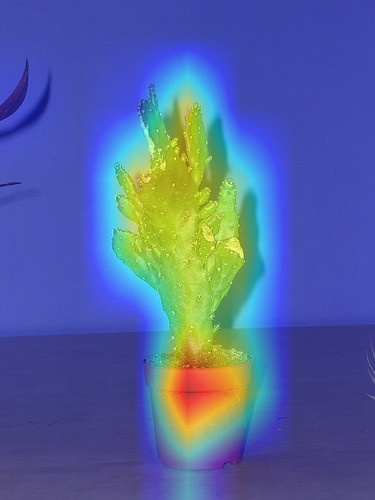
\includegraphics[width=0.20\textwidth,height=0.20\textwidth]
      {figures/val_cams/ours/2011_000145_15}
      \\
      \textbf{Car}
       & 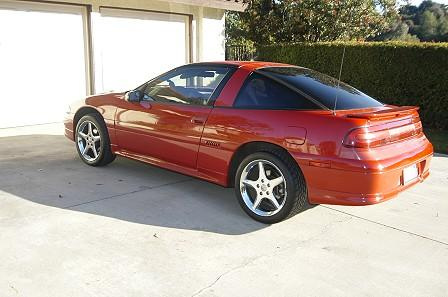
\includegraphics[width=0.20\textwidth,height=0.20\textwidth]
      {figures/originals/2010_005119}
       & 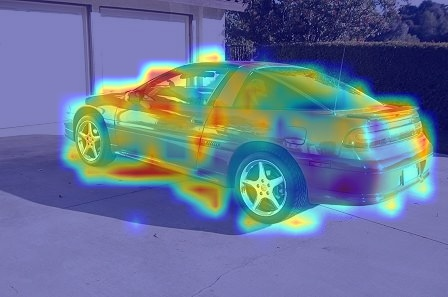
\includegraphics[width=0.20\textwidth,height=0.20\textwidth]
      {figures/val_cams/weclip/2010_005119_6}
       & 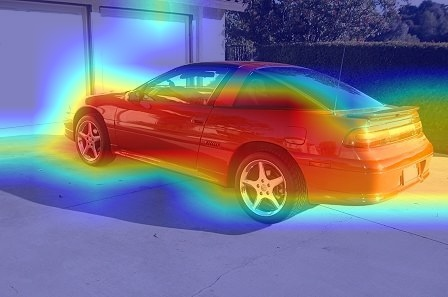
\includegraphics[width=0.20\textwidth,height=0.20\textwidth]
      {figures/val_cams/ours/2010_005119_6}
      \\
      \textbf{Bus}
       & 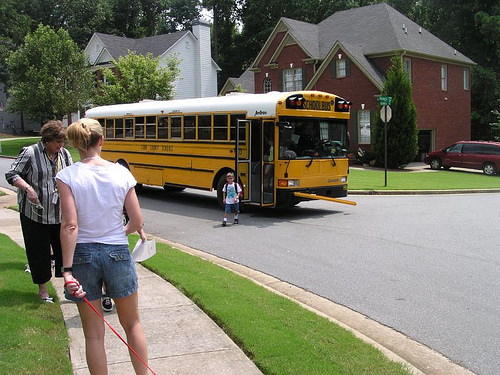
\includegraphics[width=0.20\textwidth,height=0.20\textwidth]
      {figures/originals/2010_000148}
       & 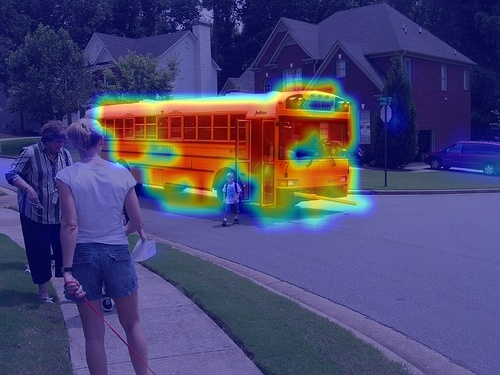
\includegraphics[width=0.20\textwidth,height=0.20\textwidth]
      {figures/val_cams/weclip/2010_000148_5}
       & 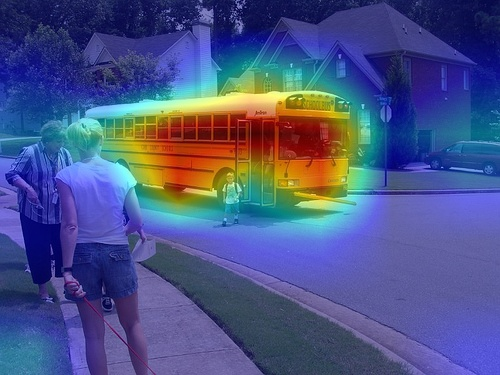
\includegraphics[width=0.20\textwidth,height=0.20\textwidth]
      {figures/val_cams/ours/2010_000148_5}
      \\
    \end{tabular}
  \end{tcolorbox}

  \caption{Qualitative comparison of CAMs between WeCLIP and our UniCL-AffSeg on PASCAL VOC 2012 \textit{val} set.}
  \label{fig:qualitative_comparison_cam_val}
\end{figure}


\begin{figure}[ht]
  \centering
  \setlength{\tabcolsep}{2pt} % adjust spacing
  \renewcommand{\arraystretch}{0.9}
  % Wrap the table in a colored box (requires \usepackage{tcolorbox})
  \begin{tcolorbox}[colframe=black!60, colback=white, boxrule=0.8pt, arc=2pt, left=2pt, right=2pt, top=2pt, bottom=2pt]
    \centering
    \begin{tabular}{cccc}
      (a) Input & (b) GT & (c) WeCLIP & (d) Ours           \\
      [1mm]

      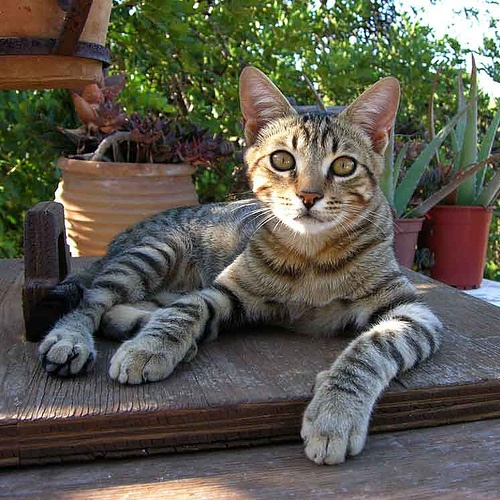
\includegraphics[width=0.20\textwidth,height=0.20\textwidth]
      {figures/originals/2007_003778}
                &
      
\includegraphics[width=0.20\textwidth,height=0.20\textwidth]
      {figures/colored_gts/2007_003778}
                &
      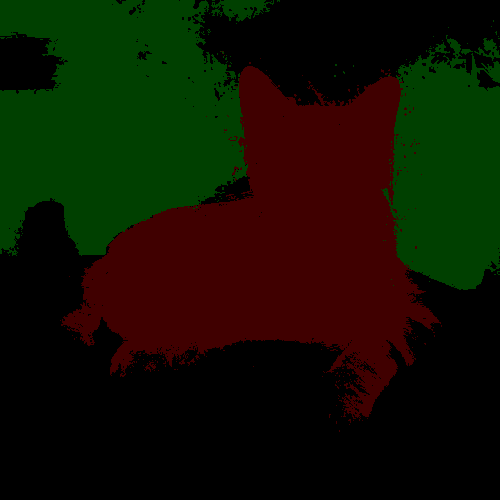
\includegraphics[width=0.20\textwidth,height=0.20\textwidth]
      {figures/val_labels/weclip/2007_003778_[7, 15]}
                &
      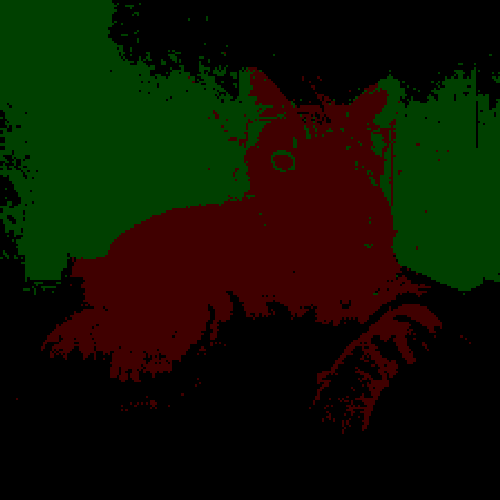
\includegraphics[width=0.20\textwidth,height=0.20\textwidth]
      {figures/val_labels/ours/2007_003778_[7, 15]}    \\

      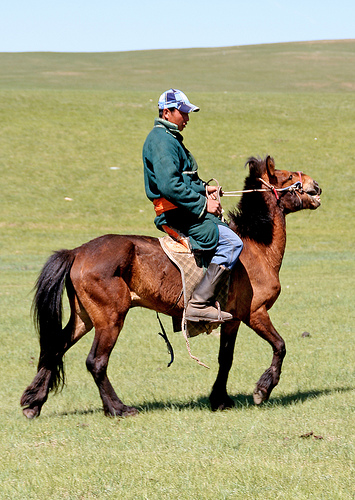
\includegraphics[width=0.20\textwidth,height=0.20\textwidth]
      {figures/originals/2009_003768}
                &
      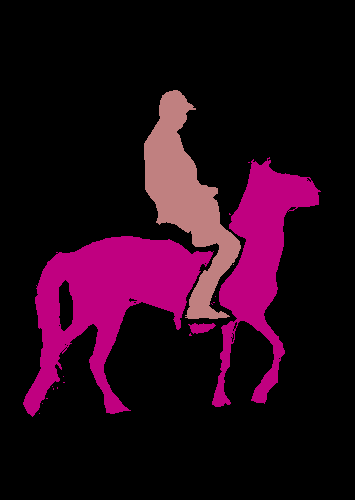
\includegraphics[width=0.20\textwidth,height=0.20\textwidth]
      {figures/colored_gts/2009_003768}
                &
      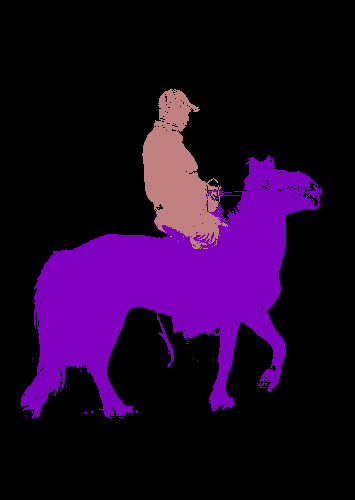
\includegraphics[width=0.20\textwidth,height=0.20\textwidth]
      {figures/val_labels/weclip/2009_003768_[12, 14]}
                &
      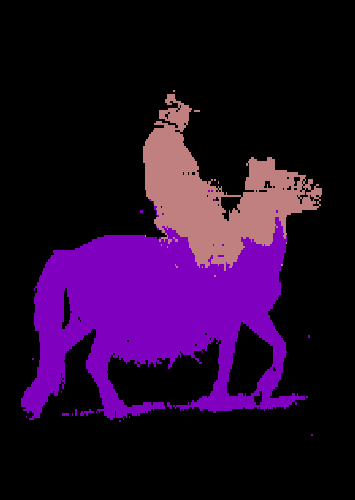
\includegraphics[width=0.20\textwidth,height=0.20\textwidth]
      {figures/val_labels/ours/2009_003768_[12, 14]}   \\

      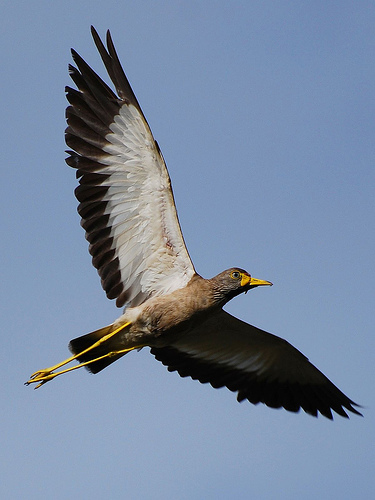
\includegraphics[width=0.20\textwidth,height=0.20\textwidth]
      {figures/originals/2011_001967}
                &
      
\includegraphics[width=0.20\textwidth,height=0.20\textwidth]
      {figures/colored_gts/2011_001967}
                &
      
\includegraphics[width=0.20\textwidth,height=0.20\textwidth]
      {figures/val_labels/weclip/2011_001967_[2]}
                &
      
\includegraphics[width=0.20\textwidth,height=0.20\textwidth]
      {figures/val_labels/ours/2011_001967_[2]}        \\


      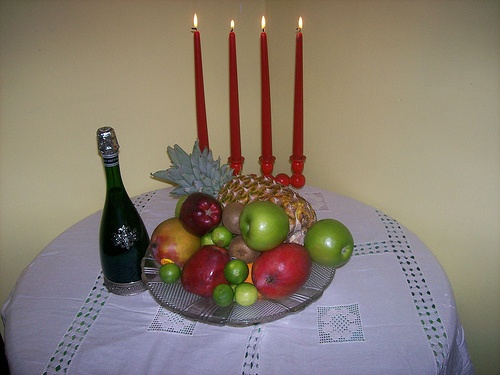
\includegraphics[width=0.20\textwidth,height=0.20\textwidth]
      {figures/originals/2007_000250}
                &
      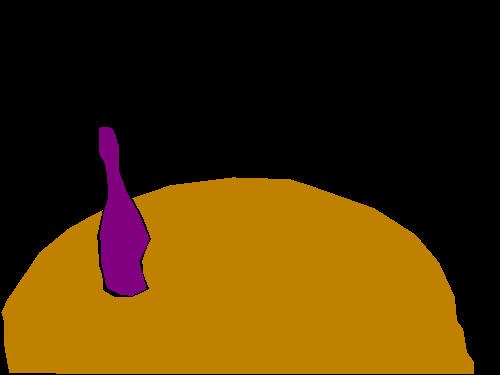
\includegraphics[width=0.20\textwidth,height=0.20\textwidth]
      {figures/colored_gts/2007_000250}
                &
      
\includegraphics[width=0.20\textwidth,height=0.20\textwidth]
      {figures/val_labels/weclip/2007_000250_[4, 10]}
                &
      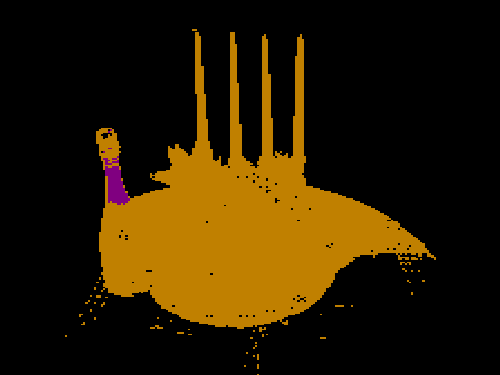
\includegraphics[width=0.20\textwidth,height=0.20\textwidth]
      {figures/val_labels/ours/2007_000250_[4, 10]}    \\


      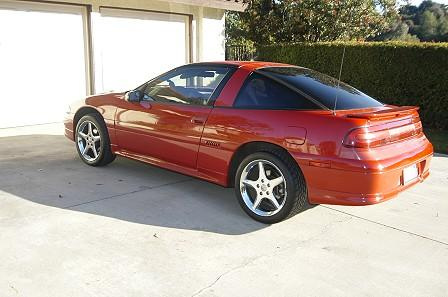
\includegraphics[width=0.20\textwidth,height=0.20\textwidth]
      {figures/originals/2010_005119}
                &
      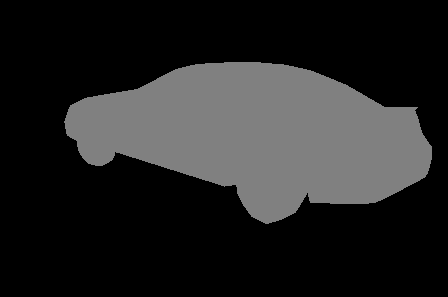
\includegraphics[width=0.20\textwidth,height=0.20\textwidth]
      {figures/colored_gts/2010_005119}
                &
      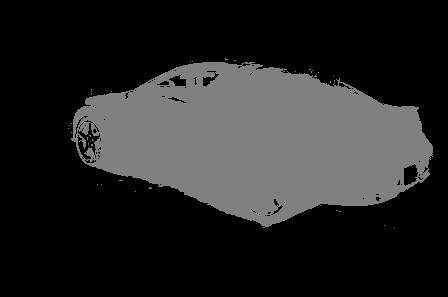
\includegraphics[width=0.20\textwidth,height=0.20\textwidth]
      {figures/val_labels/weclip/2010_005119_[6]}
                &
      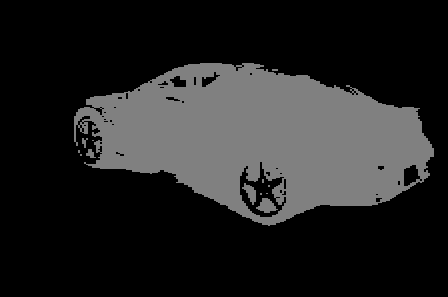
\includegraphics[width=0.20\textwidth,height=0.20\textwidth]
      {figures/val_labels/ours/2010_005119_[6]}        \\



      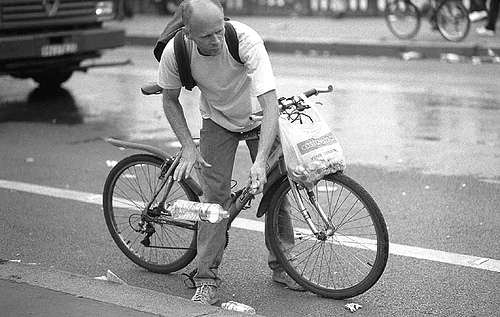
\includegraphics[width=0.20\textwidth,height=0.20\textwidth]
      {figures/originals/2011_000453}
                &
      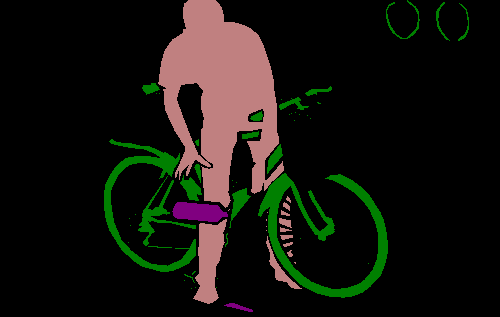
\includegraphics[width=0.20\textwidth,height=0.20\textwidth]
      {figures/colored_gts/2011_000453}
                &
      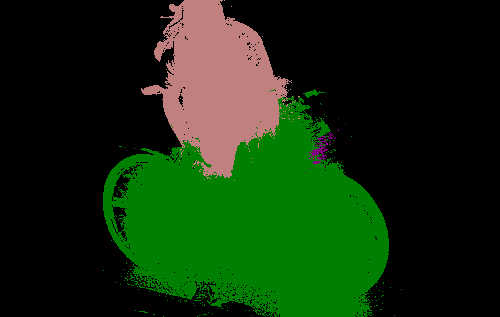
\includegraphics[width=0.20\textwidth,height=0.20\textwidth]
      {figures/val_labels/weclip/2011_000453_[1, 4, 14]}
                &
      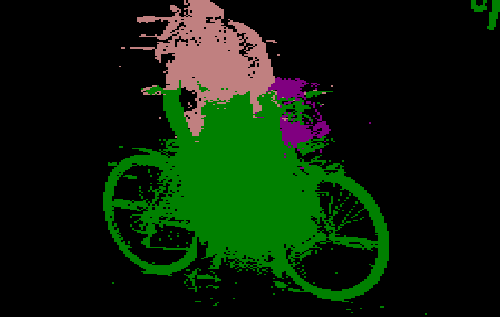
\includegraphics[width=0.20\textwidth,height=0.20\textwidth]
      {figures/val_labels/ours/2011_000453_[1, 4, 14]} \\
    \end{tabular}

    \caption{Qualitative comparison of pseudo-labels between WeCLIP and our UniCL-AffSeg on PASCAL VOC 2012 \textit{val} set.}
    \label{fig:qualitative_comparison_pseudolabel_val}
  \end{tcolorbox}
\end{figure}


\begin{figure}[ht]
  \centering
  \setlength{\tabcolsep}{2pt} % adjust spacing
  \renewcommand{\arraystretch}{0.9}
  % Wrap the table in a colored box (requires \usepackage{tcolorbox})
  \begin{tcolorbox}[colframe=black!60, colback=white, boxrule=0.8pt, arc=2pt, left=2pt, right=2pt, top=2pt, bottom=2pt]
    \centering
    \begin{tabular}{cccc}
      (a) Input & (b) GT & (c) WeCLIP & (d) (Ours)           \\
      [1mm]

      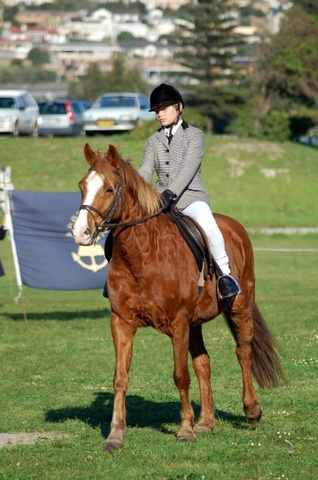
\includegraphics[width=0.20\textwidth,height=0.20\textwidth]
      {figures/originals/2007_005331}
                &
      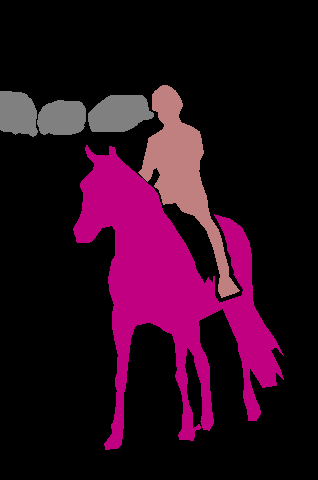
\includegraphics[width=0.20\textwidth,height=0.20\textwidth]
      {figures/colored_gts/2007_005331}
                &
      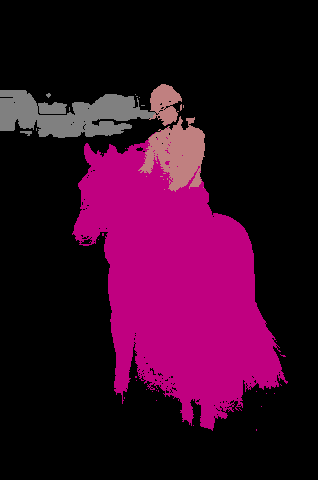
\includegraphics[width=0.20\textwidth,height=0.20\textwidth]
      {figures/test_labels/weclip/2007_005331_[6, 12, 14]}
                &
      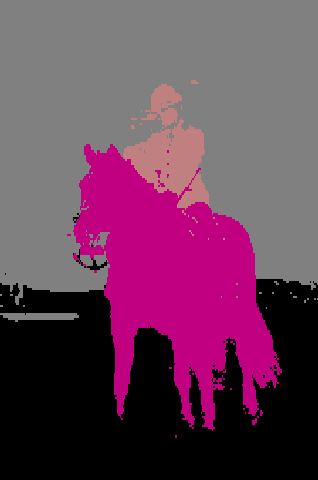
\includegraphics[width=0.20\textwidth,height=0.20\textwidth]
      {figures/test_labels/ours/2007_005331_[6, 12, 14]}    \\

      \includegraphics[width=0.20\textwidth,height=0.20\textwidth]
      {figures/originals/2007_006277}
                &
      \includegraphics[width=0.20\textwidth,height=0.20\textwidth]
      {figures/colored_gts/2007_006277}
                &
      \includegraphics[width=0.20\textwidth,height=0.20\textwidth]
      {figures/test_labels/weclip/2007_006277_[6]}
                &
      \includegraphics[width=0.20\textwidth,height=0.20\textwidth]
      {figures/test_labels/ours/2007_006277_[6]}   \\

      \includegraphics[width=0.20\textwidth,height=0.20\textwidth]
      {figures/originals/2008_001504}
                &
      \includegraphics[width=0.20\textwidth,height=0.20\textwidth]
      {figures/colored_gts/2008_001504}
                &
      \includegraphics[width=0.20\textwidth,height=0.20\textwidth]
      {figures/test_labels/weclip/2008_001504_[14]}
                &
      \includegraphics[width=0.20\textwidth,height=0.20\textwidth]
      {{figures/test_labels/ours/2008_001504_[14]}}        \\


      \includegraphics[width=0.20\textwidth,height=0.20\textwidth]
            {figures/originals/2008_002358}
                &
      \includegraphics[width=0.20\textwidth,height=0.20\textwidth]
      {figures/colored_gts/2008_002358}
                &
      \includegraphics[width=0.20\textwidth,height=0.20\textwidth]
      {figures/test_labels/weclip/2008_002358_[0]}
                &
      \includegraphics[width=0.20\textwidth,height=0.20\textwidth]
      {figures/test_labels/ours/2008_002358_[0]}    \\


      \includegraphics[width=0.20\textwidth,height=0.20\textwidth]
      {figures/originals/2009_003224}
                &
      \includegraphics[width=0.20\textwidth,height=0.20\textwidth]
      {figures/colored_gts/2009_003224}
                &
      \includegraphics[width=0.20\textwidth,height=0.20\textwidth]
      {figures/test_labels/weclip/2009_003224_[1]}
                &
      \includegraphics[width=0.20\textwidth,height=0.20\textwidth]
      {figures/test_labels/ours/2009_003224_[1]}        \\



      \includegraphics[width=0.20\textwidth,height=0.20\textwidth]
      {figures/originals/2009_004084}
                &
      \includegraphics[width=0.20\textwidth,height=0.20\textwidth]
      {figures/colored_gts/2009_004084}
                &
      \includegraphics[width=0.20\textwidth,height=0.20\textwidth]
      {figures/test_labels/weclip/2009_004084_[2]}
                &
      \includegraphics[width=0.20\textwidth,height=0.20\textwidth]
      {figures/test_labels/ours/2009_004084_[2]} \\

      
      \includegraphics[width=0.20\textwidth,height=0.20\textwidth]
      {figures/originals/2010_002531}
                &
      \includegraphics[width=0.20\textwidth,height=0.20\textwidth]
      {figures/colored_gts/2010_002531}
                &
      \includegraphics[width=0.20\textwidth,height=0.20\textwidth]
      {figures/test_labels/weclip/2010_002531_[7, 17]}
                &
      \includegraphics[width=0.20\textwidth,height=0.20\textwidth]
      {figures/test_labels/ours/2010_002531_[7, 17]} \\


    \end{tabular}

    \caption{Qualitative comparison of pseudo-labels between WeCLIP and our UniCL-AffSeg on PASCAL VOC 2012 \textit{test} set.}
    \label{fig:qualitative_comparison_pseudolabel_test}
  \end{tcolorbox}
\end{figure}


\subsection{Observations}

\subsubsection{Class Activation Maps (CAMs)}
Our UniCL-AffSeg CAMs demonstrate superior performance compared to WeCLIP in several key aspects:
\begin{itemize}
    \item \textbf{Enhanced Object Coverage and Completeness}: UniCL-AffSeg CAMs exhibit more contiguous and complete activation regions. For instance, in images such as \texttt{2007\_003778\_7.jpg} (cat) and \texttt{2011\_000453\_1.jpg} (bicycle), our CAMs capture larger, more holistic object areas, reducing sparsity and better approximating full object extents. This is attributed to the Swin-based affinity refinement, which effectively propagates activations across object parts.
    \item \textbf{Reduced Background Noise and Sharper Boundaries}: WeCLIP CAMs often include extraneous background activations, leading to noisy and diffuse maps (e.g., in \texttt{2010\_005119\_6.jpg} for car and \texttt{2010\_000148\_5.jpg} for bus). In contrast, UniCL-AffSeg CAMs show cleaner, more focused activations with sharper edges, minimizing false positives. This highlights the benefits of multi-modal fusion in UniCL over WeCLIP's ViT-only approach.
    \item \textbf{Improved Handling of Complex or Small Objects}: For challenging cases like \texttt{2011\_000145\_15.jpg} (pottedplant) and \texttt{2010\_003599\_3.jpg} (boat), UniCL-AffSeg CAMs provide finer granularity and better localization, capturing subtle details that WeCLIP misses. This is evident in multi-class images (e.g., \texttt{2007\_005702\_1.jpg}), where our method separates classes more effectively.
    \item \textbf{Consistency Across Datasets}: These improvements are consistent across both validation and test sets, with examples like \texttt{2007\_005331\_[6, 12, 14].jpg} demonstrating robustness in cluttered scenes.
\end{itemize}

\subsubsection{Pseudo-Labels}
The pseudo-labels generated by UniCL-AffSeg show marked improvements over WeCLIP, aligning more closely with ground truth annotations:
\begin{itemize}
    \item \textbf{Higher Mask Accuracy}: UniCL-AffSeg pseudo-labels capture object shapes more precisely, with fewer misclassifications or holes. For example, in \texttt{2007\_003778\_[7, 15].png} (cat and person), our masks outperform WeCLIP's fragmented outputs.
    \item \textbf{Finer Boundary Delineation}: Our pseudo-labels exhibit cleaner, more defined edges, reducing noise and over-segmentation. In test examples like \texttt{2008\_001504\_[14].png} (horse) and \texttt{2009\_003224\_[1].png}, WeCLIP produces noisy masks, while UniCL-AffSeg yields smoother, more accurate boundaries.
    \item \textbf{Better Performance on Diverse Scenarios}: Trends hold for easy (e.g., \texttt{2011\_001967\_[2].png} for bird) and hard cases (e.g., \texttt{2010\_005119\_[6].png} for car), with UniCL-AffSeg narrowing the gap to fully supervised methods. Limitations persist for highly occluded or tiny objects (e.g., \texttt{2007\_000250\_[4, 10].png}).
    \item \textbf{Cross-Set Generalization}: Similar gains are observed in test labels, such as \texttt{2009\_004084\_[2].png}, underscoring boundary precision and completeness.
\end{itemize}

Overall, these qualitative results underscore UniCL-AffSeg's advantages in weakly supervised semantic segmentation, driven by its Swin transformer backbone and affinity-based refinement. This supports the quantitative improvements (e.g., higher mIoU) reported in the results section, demonstrating UniCL-AffSeg's potential to bridge the gap with fully supervised approaches.





\subsection{Per-Class Performance Analysis}
\label{subsec:per_class_performance_analysis}

To gain a deeper understanding of our model’s behavior, we analyzed the per-class Intersection over Union (IoU) scores on the PASCAL VOC 2012 validation set. This analysis highlights how the model performs across different object categories, providing insights beyond the overall metrics.

\subsubsection{High-Performing Classes}

Classes with a large spatial extent and higher representation in the dataset achieve relatively high IoU scores. For instance, \textbf{background} (77.8\%), \textbf{bus} (67.5\%), \textbf{cat} (65.9\%), and \textbf{dog} (65.1\%) are segmented effectively. These results indicate that the model can reliably capture dominant objects with distinctive visual features.

\subsubsection{Low-Performing Classes}

In contrast, smaller or less frequent classes such as \textbf{person} (16.9\%), \textbf{chair} (25.3\%), and \textbf{potted plant} (28.3\%) exhibit lower IoU scores. This suggests that the model struggles with rare or small objects, likely due to their limited representation in the training set and small spatial footprint in the images.

\subsubsection{Observations}

Overall, the model performs better on large and visually distinctive classes such as animals and vehicles, while it underperforms on humans, furniture, and small objects. These per-class performance results provide valuable insights that can guide future improvements, such as incorporating multi-scale features or class-specific data augmentation to better handle challenging classes.


\begin{table}[ht]
\centering
\caption{Per-Class IoU Performance on PASCAL VOC (Latest Results)}
\begin{tabular}{|c|l|c|}
\hline
\textbf{Index} & \textbf{Class}      & \textbf{IoU} \\ \hline
0  & background   & 0.7784  \\
1  & aeroplane    & 0.5685  \\
2  & bicycle      & 0.3191  \\
3  & bird         & 0.6044  \\
4  & boat         & 0.4360  \\
5  & bottle       & 0.3677  \\
6  & bus          & 0.6753  \\
7  & car          & 0.4881  \\
8  & cat          & 0.6591  \\
9  & chair        & 0.2525  \\
10 & cow          & 0.5887  \\
11 & diningtable  & 0.4041  \\
12 & dog          & 0.6511  \\
13 & horse        & 0.6132  \\
14 & motorbike    & 0.5846  \\
15 & person       & 0.1697  \\
16 & pottedplant  & 0.2828  \\
17 & sheep        & 0.6305  \\
18 & sofa         & 0.4661  \\
19 & train        & 0.5642  \\
20 & tvmonitor    & 0.4032  \\ \hline
\end{tabular}
\end{table}

\begin{table}[ht]
\centering
\caption{Overall Performance Metrics}
\begin{tabular}{|l|c|}
\hline
\textbf{Metric} & \textbf{Value} \\ \hline
Pixel Accuracy (pAcc) & 0.7981 \\
Mean Accuracy (mAcc)  & 0.6997 \\
Mean IoU (mIoU)       & 0.5003 \\ \hline
\end{tabular}
\end{table}

% The model achieved a mean IoU of 0.5003 on the PASCAL VOC dataset, with a pixel accuracy of 0.7981 and a mean accuracy of 0.6997. Performance varies significantly across classes: large and well-represented classes such as \textbf{background} (0.7784), \textbf{bus} (0.6753), \textbf{cat} (0.6591), and \textbf{dog} (0.6511) are segmented effectively, while smaller or less frequent classes like \textbf{person} (0.1697), \textbf{chair} (0.2525), and \textbf{potted plant} (0.2828) remain challenging. These results suggest that while the model captures the dominant classes well, further improvements are needed to better handle rare and small objects.
\section{Ablation Study}
\label{sec:ablation_study}
\begin{table}[h!]
\centering
\begin{tabular}{|l|c|}
\hline
\textbf{Class} & \textbf{IoU} \\
\hline
background    & 0.79597609 \\
aeroplane     & 0.60649828 \\
bicycle       & 0.24300995 \\
bird          & 0.56525227 \\
boat          & 0.41434259 \\
bottle        & 0.39108619 \\
bus           & 0.63887711 \\
car           & 0.41678079 \\
cat           & 0.52468153 \\
chair         & 0.24156961 \\
cow           & 0.57364590 \\
diningtable   & 0.31857660 \\
dog           & 0.56249454 \\
horse         & 0.56194598 \\
motorbike     & 0.53527557 \\
person        & 0.21941806 \\
potted plant  & 0.28315749 \\
sheep         & 0.59557354 \\
sofa          & 0.37300971 \\
train         & 0.53391481 \\
tv/monitor    & 0.45051146 \\
\hline
\textbf{Mean IoU (mIoU)} & \textbf{0.46883800} \\
\hline
\end{tabular}
\caption{Per-class IoU and mIoU for Pascal VOC without RFM.}
\label{tab:pascal_first_set_miou}
\end{table}


